\chapter{Reference implementation}
\label{ch:implementation}

\section{Project Setup}
\label{sec:project-setup}

The underlying \emph{server infrastructure} for the reference implementation was an existing server with 16 \ac{CPU}-cores (with multithreading), 64 \ac{GB} \ac{RAM} and a 512 \ac{GB} \ac{SSD} drive, located on the \ac{JGU} campus and connected to the internet via a dedicated one-gigabit network connection (see speedtest\footnote{\url{https://www.speedtest.net/}} results in \autoref{listing:speedtestServer}).

\begin{listing}[!ht]
\inputminted{text}{04_Artefakte/03_Listings/speedtest-server.txt}
\caption{Speedtest showing connection statistics for the server used to deploy the application\protect}
\label{listing:speedtestServer}
\end{listing}

The orchestration was deployed first to allow development on a working remote WebRTC infrastructure.
The basis was a clean, freshly bootstrapped Kubernetes installation running on the bare-metal server.
LiveKit and its Redis database were installed via the application deployment manager Helm, using an official installation chart published by its maintainers\footnote{\url{https://github.com/livekit/livekit-helm}}.
To simplify the deployment, LiveKit was placed behind the reverse proxy Traefik\footnote{\url{https://traefik.io/}} to manage \ac{SSL} termination via the LetsEncrypt\footnote{\url{https://letsencrypt.org/}} service and routing to the actual service running inside the cluster.
The potential downside of this deployment configuration was deemed insignificant since the server only needs to service a handful of users.
The detailed Kubernetes setup instructions are documented in the according folder in the project\textquotesingle s repository.

The \emph{LiveKit} installation was deployed with only a slight deviation from the default configuration.
It was set up to use \ac{TCP} as a transport protocol instead of exposing a range of UDP ports to allow easier integration with \ac{SSL} termination using the reverse proxy.
Otherwise, the configuration defined the endpoints for sending webhook requests and custom credentials for making requests to it via the server-side \ac{SDK} and generating valid access tokens for users to connect to rooms.
The Helm installation chart was used to set up the system along with its Redis database installation in a single command, and the server was immediately ready for connections.

The development process was conducted in a desktop environment using the suite of tools developed by JetBrains\footnote{\url{https://www.jetbrains.com/}} (WebStorm, PyCharm and CLion), as these are free for educational use and provide a comprehensive environment for development, including debugging, intelligent code completion, versioning, containerisation and deployment.
A Docker Desktop installation allowed running services and databases locally to support development before publishing to the production environment.
Versioning was done via Git\footnote{\url{https://git-scm.com/}} on the GitLab platform provided by the \ac{JGU}\footnote{\url{https://gitlab.rlp.net}}.

\section{API server}
\label{sec:api-server}

The first custom implementation, the \ac{API} server, was generated using the Feathers \ac{CLI} tool with standard username and password authentication and WebSockets and \ac{HTTP} transports enabled.
It provides the core services for Users, Spaces, Tokens and LiveKit events.
These services were autogenerated using the Feathers \ac{CLI} utility.
They were used largely unmodified, except for adding the properties on the models for Users and Spaces as defined in \autoref{sec:datamodeling}.
A custom service class was added for the Tokens, as these do not persist in the database and instead are generated on the fly by the LiveKit server \ac{SDK}.
All other boilerplate code for the \ac{API}, including the MongoDB integration, the authentication mechanism, and the REST and WebSockets transport integrations, was also autogenerated using the \ac{CLI}.
An additional custom Livekit event service was added to the API, allowing it to receive webhook requests via \ac{HTTP} from the LiveKit server containing updates on connecting and disconnecting users.
These events do not persist in the database but are relayed to the connected users via real-time channels.
The channels feature provided by Feathers was used to automatically subscribe connecting users to updates on the services for Spaces and Livekit events.

\section{Core SDK}
\label{sec:core-sdk}

The basic functionality was bundled in an \ac{NPM} module to make the base code independent of the use case, which could later be used in other projects.
This module contains the abstract classes \textquote{DataProducer}, \textquote{HeadTracker} and \textquote{SonificationController} alongside the message specification for the various types of transmitted data.
It was written to propagate updates via events instead of the reactive patterns used in Vue so that it can also be used independently from the framework used for the study.
Unit tests were added to the module to maintain a stable implementation, providing sufficient test coverage with only a few branches left uncovered that were deemed insignificant (see \autoref{listing:sdkCoverage}).

\begin{listing}[!ht]
\inputminted{text}{04_Artefakte/03_Listings/sdk-test-coverage.txt}
\caption{SDK test coverage report\protect}
\label{listing:sdkCoverage}
\end{listing}

\section{User interface}
\label{sec:user-interface}

The Quasar framework provides a \ac{CLI} to generate new projects, which allows selecting basic implementation details (e.g.\ language, state management) and producing a complete and working empty Vue project with sample components that served as the starting point for the \ac{UI} implementation.
The first thing added to the project was the library feathers-pinia\footnote{\url{https://feathers-pinia.pages.dev}}, which is provided by the Feathers developer community and promises easy integration of an existing Feathers \ac{API} with any Vue project using the Pinia\footnote{\url{https://pinia.vuejs.org/}} state management system used by Vue.
The extension was integrated by linking the client library that the Feathers server project automatically generates by referencing the \ac{API}\textquotesingle s project folder and configuring basic authentication settings.
The routing configuration and page components were set up according to the sitemap (\autoref{fig:uiSitemap}).

\begin{figure}[!ht]
\includesvg[width=\textwidth]{04_Artefakte/01_Abbildungen/ui-sitemap}
\caption[Sensorama UI sitemap]{Sitemap for the Sensorama UI\protect}
\label{fig:uiSitemap}
\end{figure}

The overview page for the spaces presents a list of the names alongside the currently connected users and buttons to either join as a participant or passively view it as a spectator.
On joining a space, the user must first activate their microphone to activate the audio context.
The user is then presented with three basic control panels (see \autoref{fig:screenshotJoin}).
The \textquote{Data producer} panel allows setting a URL of a local WebSockets server of a data producer, setting the message type received from it, and optionally enabling a tracing function to log the packet transmission statistics.
Once connected, the panel shows a preview of the incoming points data, transmission statistics and a button to disconnect.
Internally, the panel creates a reactive data store that instantiates the \textquote{DataProducer} class from the core \ac{SDK}, watches incoming message events and populates the received data as reactive properties to be used across the \ac{UI} in various other components without the need to create additional class instances.
The second panel, \textquote{Head tracker}, works similarly but uses the Web Bluetooth \ac{API} to select a nearby device and connects to it to receive its data messages.
The third component configures the sonification by setting thresholds on incoming movement quality values.
It connects to an instance of the \textquote{SonificationController} class from the core \ac{SDK} and allows the configuration of event thresholds, sound selection and harmonic configuration.

\begin{figure}[!ht]
\centering
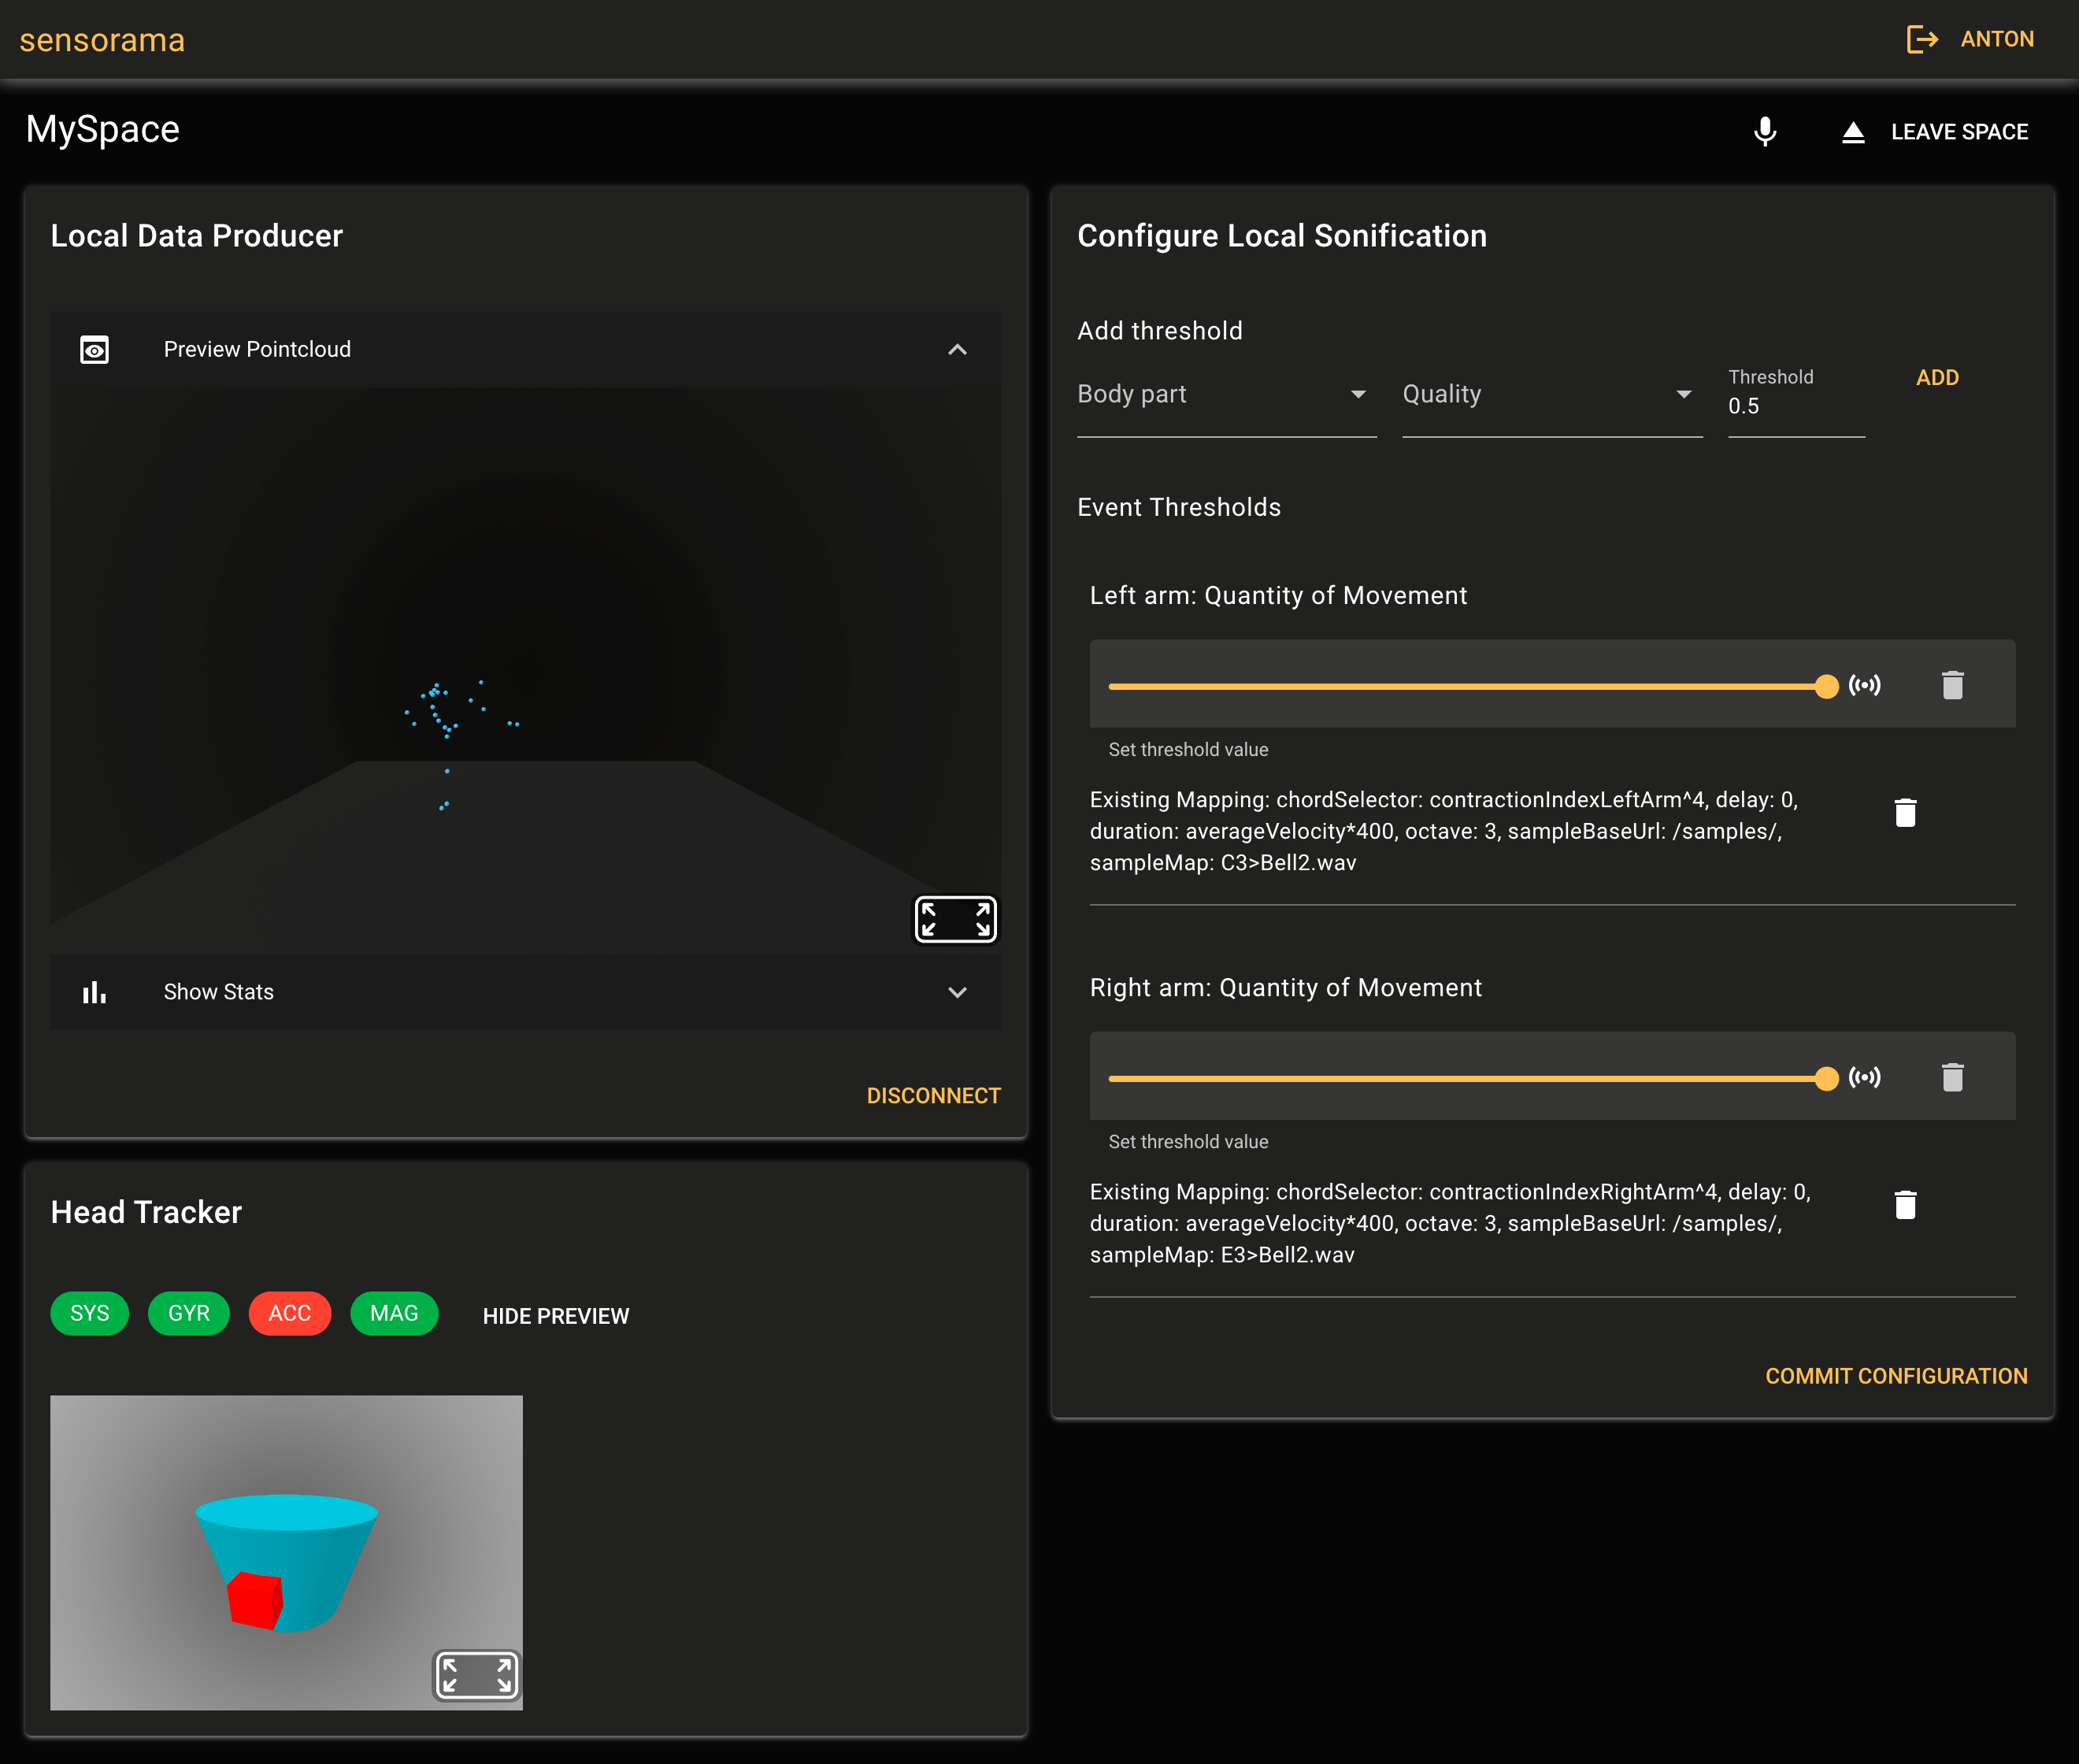
\includegraphics[width=\textwidth]{04_Artefakte/01_Abbildungen/screenshot-join}
\caption[Join space page screenshot]{Page layout when joining a space as a participant\protect}
\label{fig:screenshotJoin}
\end{figure}

When using the page to view a space  (see \autoref{fig:screenshotView}), there is only one component, the \textquote{SpaceViewer}, that shows a \ac{3D} room in which all incoming points are rendered as small spheres, giving the impression of a human figure.
For each participant, there is a differently coloured light source that follows the centre of mass of the points associated with the participant.
The viewer also renders all sonifications and audio streams at their respective spatial positions.
This allows the user to view the \ac{3D} scene on screen while listening to binaural audio or to use the built-in \ac{VR} functionality to experience the scene in a visually immersive way.

\begin{figure}[!ht]
\centering
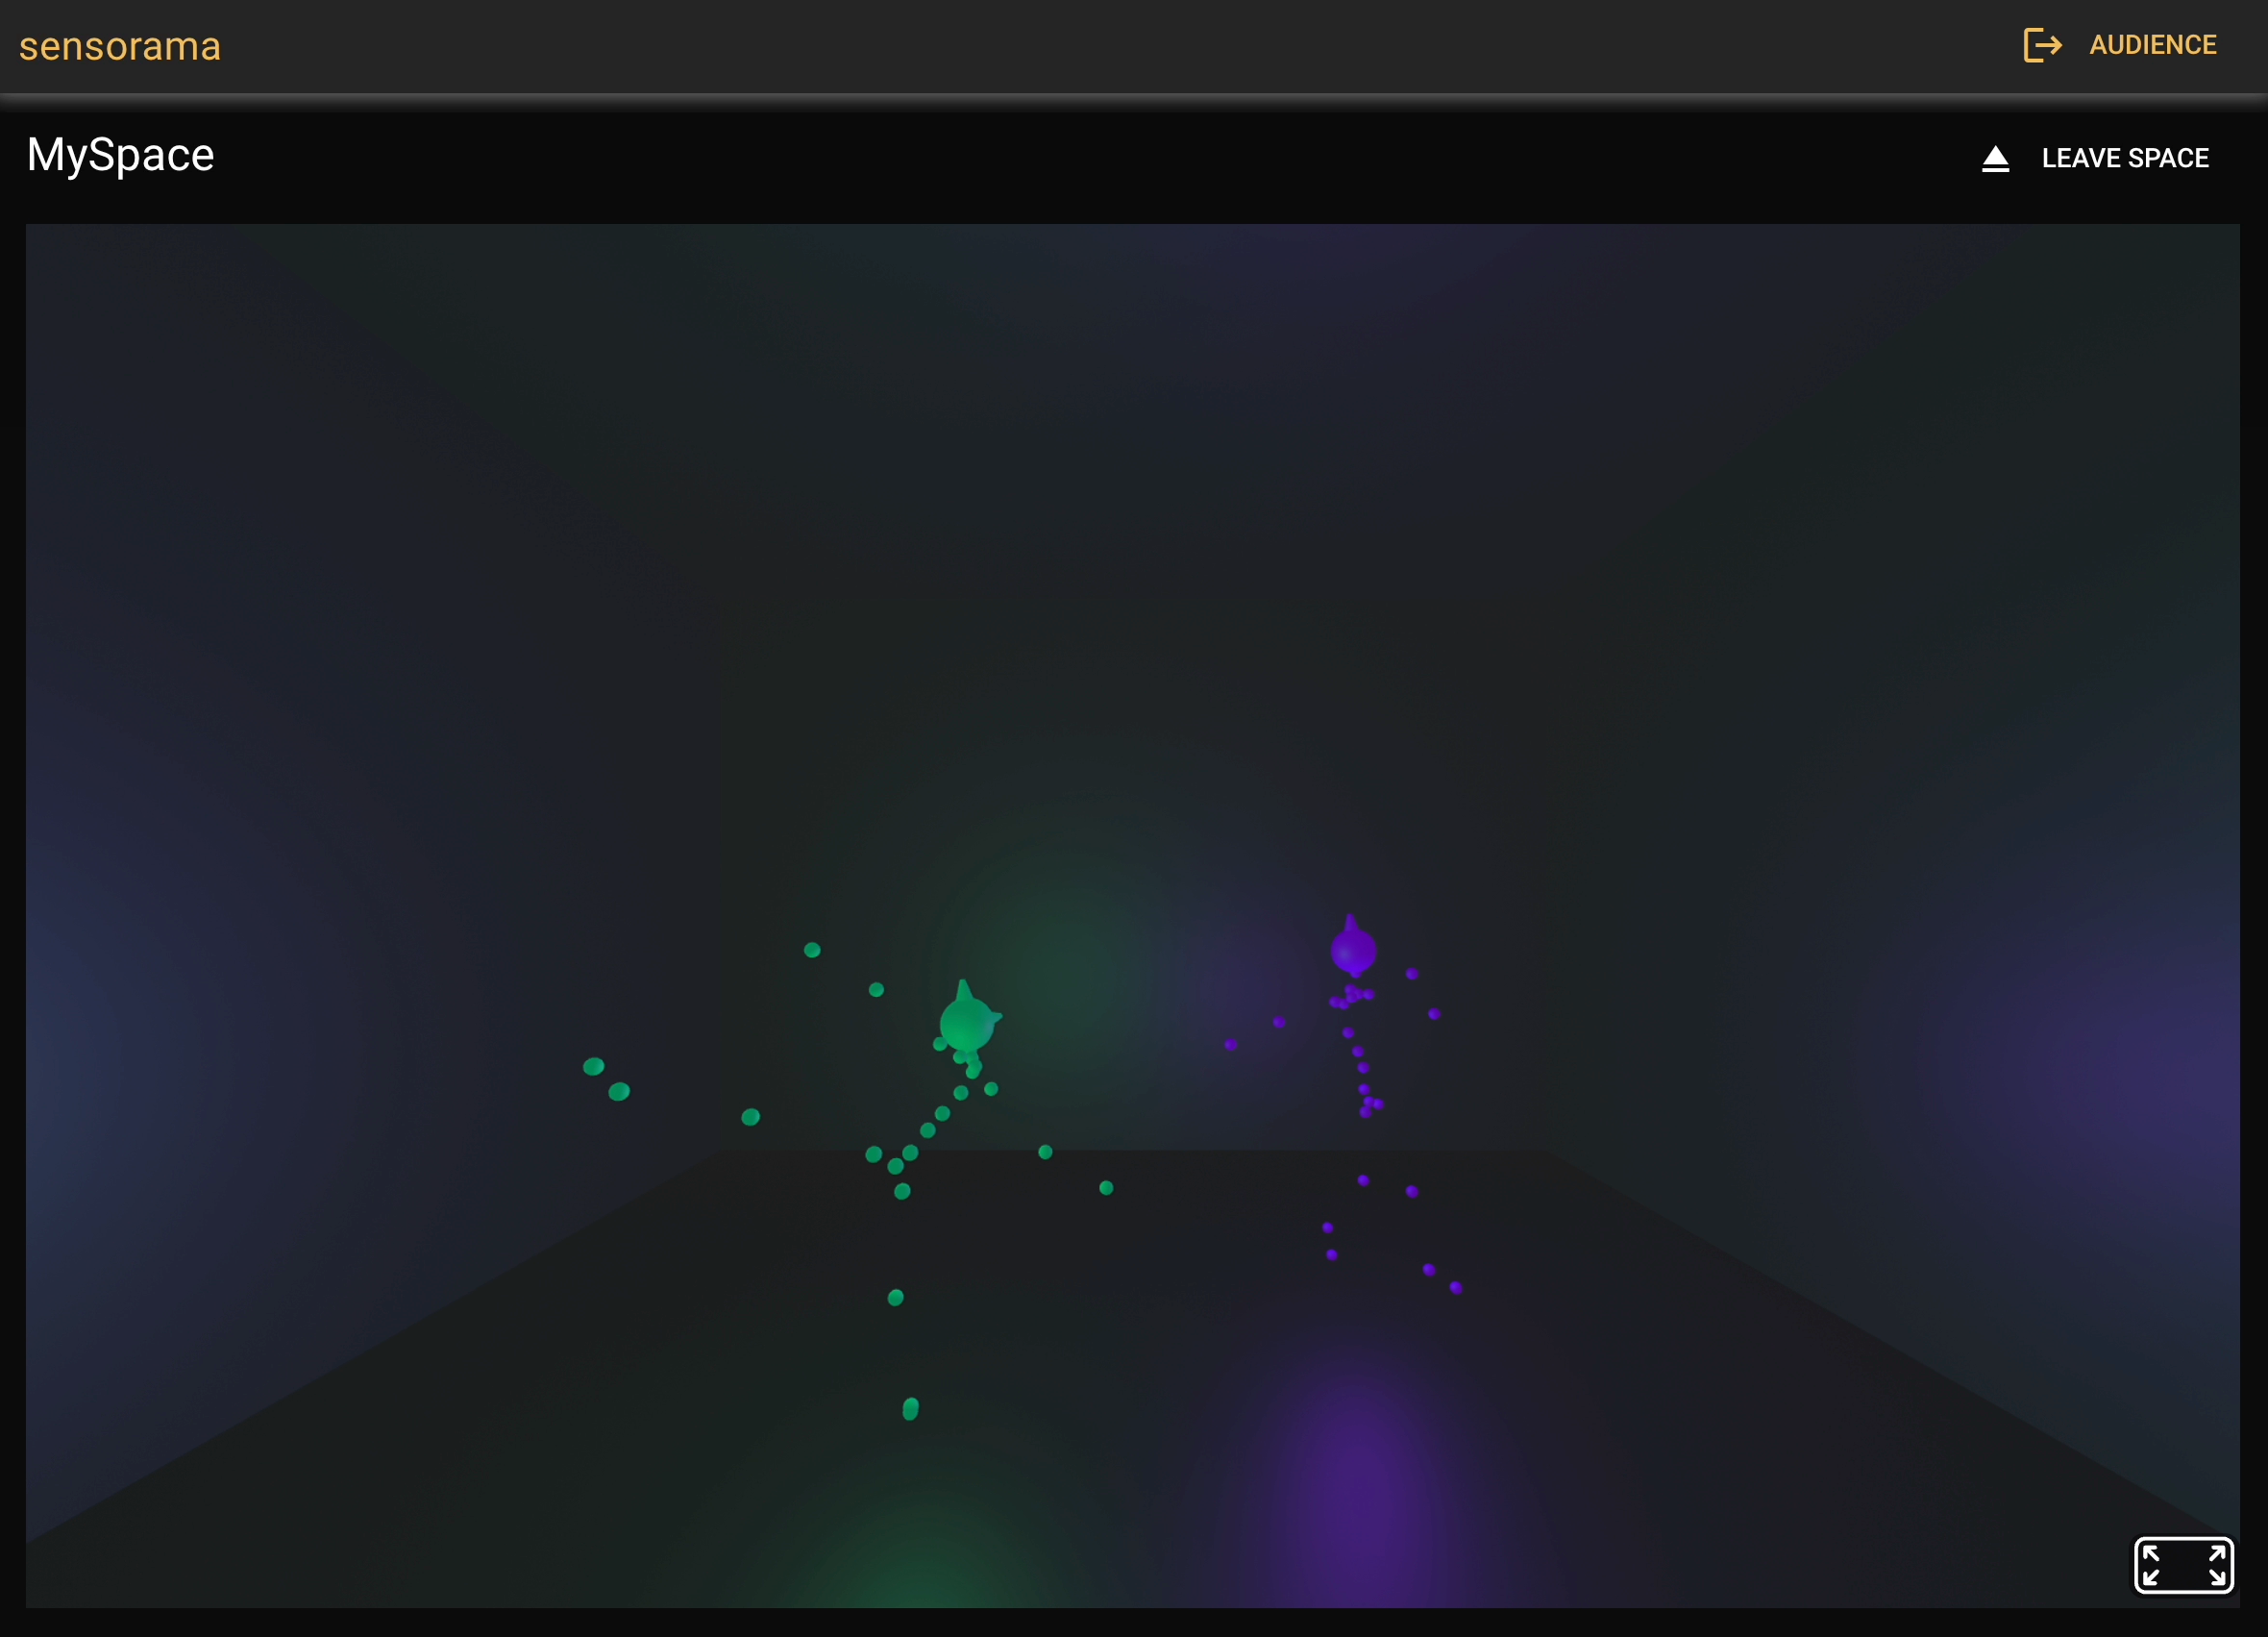
\includegraphics[width=\textwidth]{04_Artefakte/01_Abbildungen/screenshot-view}
\caption[View space page screenshot]{Page layout when passively viewing a space\protect}
\label{fig:screenshotView}
\end{figure}

\section{Data producers}
\label{sec:data-producers}

The general \emph{data producer} was written in Python and provides multiple data sources: an interface to a Blazepose implementation on the Oak-D \ac{3D} camera, as well as reading depth images as point clouds from the camera and an interface to load and playback motion capture data in the \ac{BVH} file format.
All three data sources were implemented as separate Python classes because the classes related to the Oak-D camera were built by modifying existing code for pose recognition~\parencite{githubDepthAiBlazePose} and point cloud processing~\parencite{githubDepthAiPointcloud}.
The \ac{BVH} data source was created from scratch and implemented to facilitate testing and development by using playback of motion capture data of professional dancers pre-recorded on the Captury Live system.
All data source classes were set up to support calling a function in a loop and returning current point data as a multidimensional array.
The returned data is packed as a byte sequence and sent to the connected browser over WebSockets in the appropriate format (see \autoref{sec:datamodeling}).
This way, the disparate sources could be imported into a single central file that uses a combined set of utility functions for running a WebSockets server and packing data.
Due to the lack of a Python-based client for the Captury Live system, the Captury producer had to be implemented separately as a C++ project using CMake\footnote{\url{https://cmake.org/}} as a build system and based on the \textquote{RemoteCaptury} client library~\parencite{githubRemoteCaptury}, as well as an example project for a WebSockets server implementation in C++~\parencite{githubCppWebSocketsDemo}.

The custom-built head-tracking device was implemented as an Arduino project.
As such, it was first realised as a hardware setup (\autoref{fig:headTrackerAssembled}) and then outfitted with custom firmware written in the Arduino-specific flavour of C/C+.
The hardware implementation was created using the \textquote{Arduino Connect RP2040}\footnote{\url{https://docs.arduino.cc/hardware/nano-rp2040-connect/}}, which is based on the Raspberry PI 2040 microcontroller and has an onboard BluetoohLE module.
The \ac{IMU} module used was the \textquote{9-DOF Absolute Orientation IMU Fusion Breakout}\footnote{\url{https://www.adafruit.com/product/4646}} which uses the BNO055\footnote{\url{https://www.bosch-sensortec.com/products/smart-sensor-systems/bno055/}} chip produced by Bosch.
This chip already pre-processes the data from the gyroscope, accelerometer and magnetometer into an absolute world position that can be directly read from the breakout board via the \ac{I2C} bus.
As a third component, a small 3.7V lithium battery was added alongside a charging module\footnote{\url{https://www.adafruit.com/product/1905}}.
Only six connections needed to be soldered between the three modules (2x charger and 4x \ac{IMU}), and the resulting circuit was ready to function as a custom head tracker (\autoref{fig:headTrackerWiring}).
For the software implementation, the basic example code for the Adafruit module was used to set up continuous polling of the positioning module, reading the values for position and device calibration status and sending them as byte sequences at a fixed rate of ~25fps over BluetoothLE\@.

\begin{figure}[!ht]
\centering
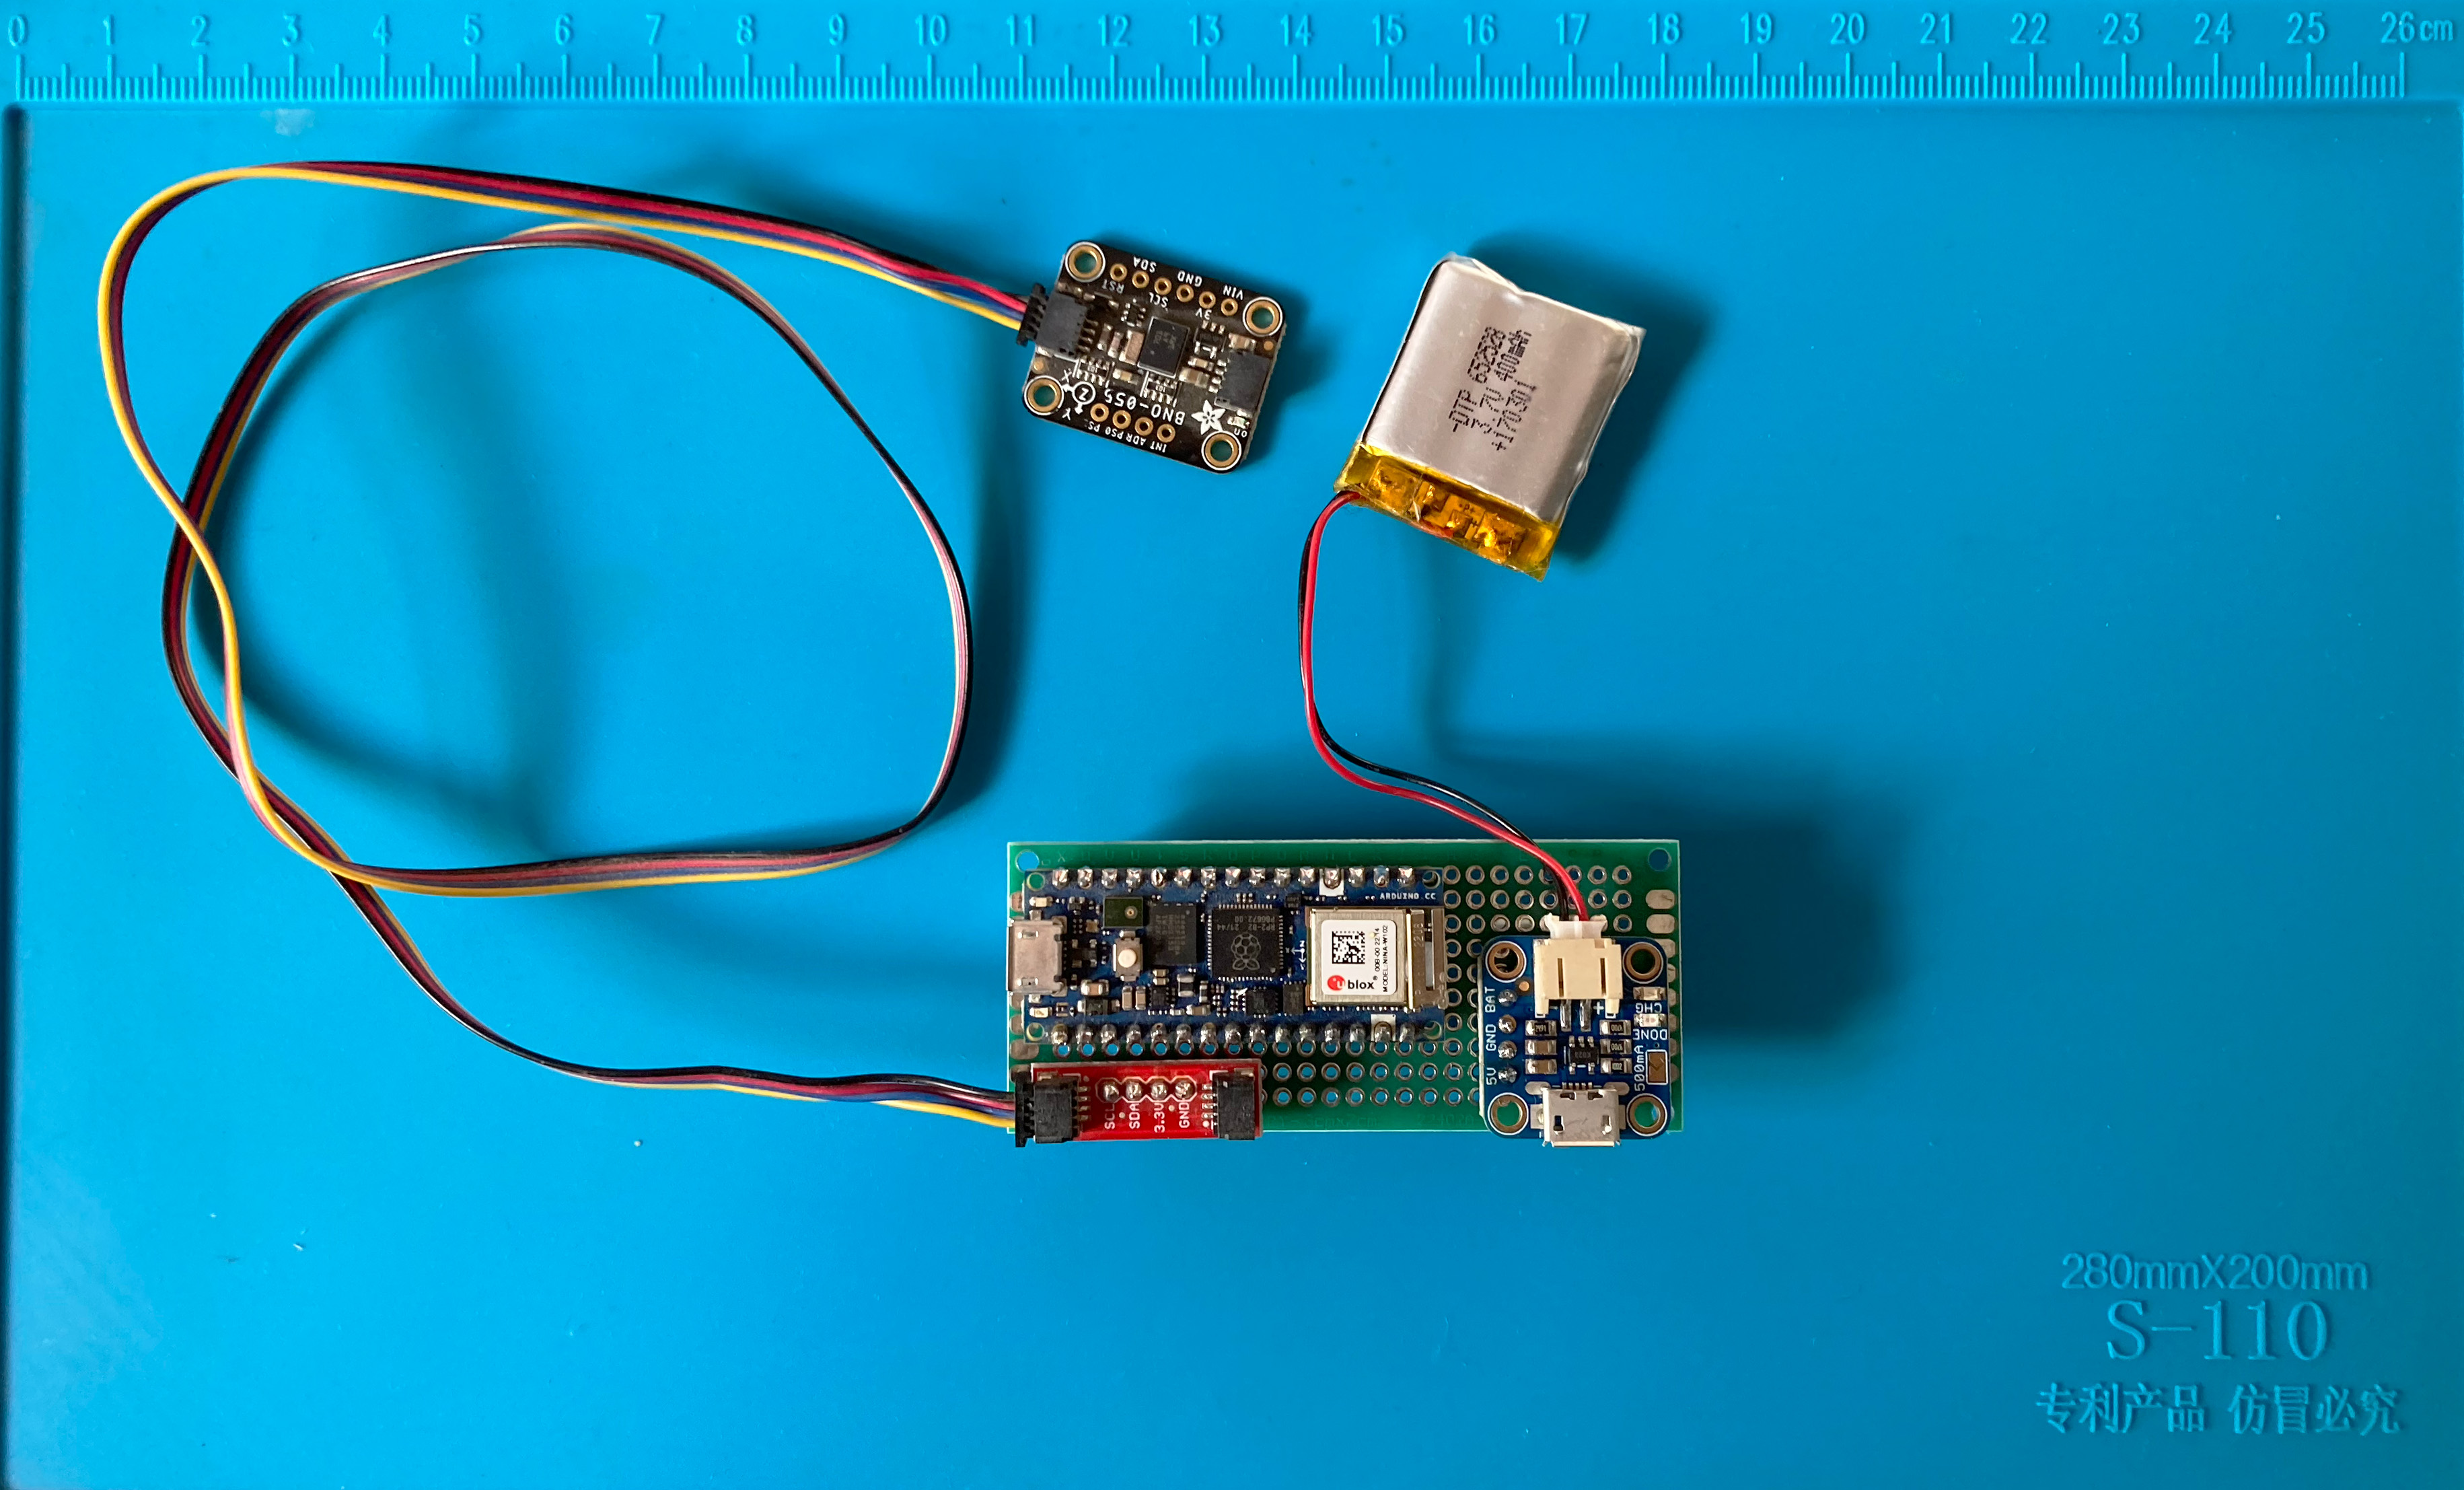
\includegraphics[width=\textwidth]{04_Artefakte/01_Abbildungen/head-tracker-photo}
\caption[Example assembled head tracker]{Example head tracker assembly\protect}
\label{fig:headTrackerAssembled}
\end{figure}

\begin{figure}[!ht]
\centering
\includesvg[scale=1.0]{04_Artefakte/01_Abbildungen/head-tracker-wiring}
\caption[Head tracker wiring diagram]{Wiring diagram for the custom head tracker\protect}
\label{fig:headTrackerWiring}
\end{figure}
